\documentclass[a4paper,class=article,border=5pt,tikz]{standalone}

\begin{document}

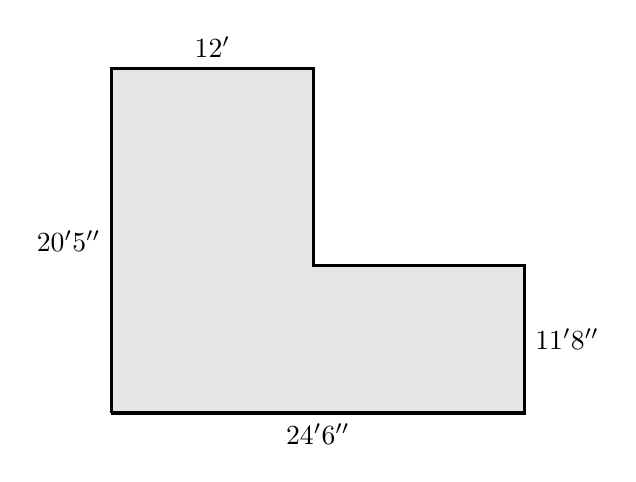
\begin{tikzpicture}[thick,scale=0.2]
% 20'5'' = 245'' = 622.3cm
% 12'    = 144'' = 365.76cm
% 11'8'' = 140'' = 355.6cm
% 24'6'' = 294'' = 746.76cm
% 622.3-355.76 = 266.54cm
\draw [very thick, fill=gray!20](0,0) -- (0,622.3pt) node[midway,left]{$20'5''$} -- (365.76pt,622.3pt) node[midway,above]{$12'$} -- (365.76pt,266.54pt) -- (746.76pt,266.54pt) -- (746.76pt,0pt) node[midway,right]{$11'8''$} -- (0,0) node[midway,below]{$24'6''$};
\end{tikzpicture}

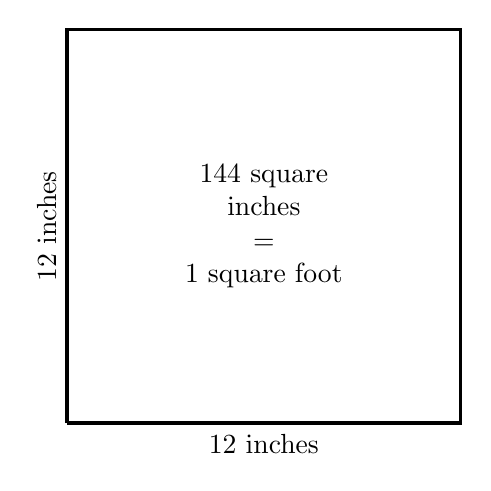
\begin{tikzpicture}[thick, sharp corners, scale=5]
\draw [very thick](0,0) -- (0,1) node[above,midway,rotate=90]{$12$~inches} -- (1,1) -- (1,0) -- (0,0) node[below,midway]{$12$~inches};
\node at (0.5,0.5) {\parbox{2cm}{\centering$144$~square inches\\$=$\\$1$~square foot}};
\end{tikzpicture}

\end{document}

